\documentclass[conference]{IEEEtran}
\IEEEoverridecommandlockouts
% The preceding line is only needed to identify funding in the first footnote. If that is unneeded, please comment it out.
\usepackage{cite}
\usepackage{amsmath,amssymb,amsfonts}
\usepackage{algorithmic}
\usepackage[ruled,vlined]{algorithm2e}
\usepackage{pgfplots}
\usepackage{graphicx}
\graphicspath{{../images}}
\usepackage{textcomp}
\usepackage{xcolor}
\usepackage{verbatim}
\def\BibTeX{{\rm B\kern-.05em{\sc i\kern-.025em b}\kern-.08em
    T\kern-.1667em\lower.7ex\hbox{E}\kern-.125emX}}
\begin{document}

\title{Unsupervised Learning of Visual Features by Contrasting Cluster Assignments}

\author{\IEEEauthorblockN{Seri Lee}
\IEEEauthorblockA{\textit{Computer Science and Engineering} \\
\textit{Seoul National University}\\
Seoul, Republic of Korea\\
sally20921@snu.ac.kr} 
}

\maketitle

\begin{abstract}
Unsupervised image representations have significantly reduced the gap with supervised pretraining, notably with the recent achievements of contrastive learning methods.
These contrastive methods typically work online and rely on a large number of explicit pairwise feature comparisons, which is computationally challenging.
In this paper, we propose an online algorithm, SwAV, that takes advantage of contrastive methods without requiring to compute pairwise comparisons. 
Specifically, our method simultaneously clusters the data while enforcing consistency between cluster assignments produced for different augmentations (or "views") of the same image, instead of comparing features directly as in contrastive learning.
Simply put, we use a "swapped" prediction mechanism where we predict the code of a view from the representation of another view.
Our method can be trained with large and small batches and can scale to unlimited amounts of data. 
Compared to previous contrastive methods, our method is more memory efficient since it does not require a large memory bank or a special momentum network.
In addition, we also propose a new data augmentation strategy, multi-crop, that uses a mix of views with different resolutions in place of two full-resolution views, without increasing the memory or compute requirements.
We validate our findings by achieving 75.3\% top-1 accuracy on ImageNet with ResNet-50, as well as surpassing supervised pretraining on all the considered transfer tasks.
\end{abstract}

\section{Introduction}
\cite{b1}.

Unsupervised visual representation learning, or self-supervised learning, aims at obtaining features without using manual annotations and is rapidly closing the performance gap with supervised pretraining in computer vision.
Many recent state-of-the-art methods build upon the instance discrimination task that considers each image of the dataset (or ``instance'') and its transformations as a separate class.
This task yields representations that are able to discriminate between different images, while achieving some invariance to image transformations.
Recent self-supervised methods that use instance discrimination rely on a combination of two elements: (1) a contrastive loss and (2) a set of image transformations.
The contrastive loss removes the notion of instance classes by directly comparing image features while the image transformations define the invariances encoded in the features.
Both elements are essential to the quality of the resulting networks and our work improves upon both the objective function and the transformations.

The contrastive loss explicitly compares pairs of image representations to push away representations from different images while pulling together those from transformations, or views, of the same image.
Since computing all the pairwise comparisons on a large dataset is not practical, most implementations approximate the loss by reducing the number of comparisons to random subsets of images during training.
An alternative to approximate the loss is the approximate the task-that is to relax the instance discrimination problem. 
For example, clustering-based methods discriminate between groups of images with similar features instead of individual images. 
The objective in clustering is tractable, but it does not scale well with the datasets as it requires a pass over the entire dataset to form image ``codes'' (\textit{i.e.}, cluster assignments) that are used as targets during training.
In this work, we use a different paradigm and propose to compute the codes online while enforcing consistency between codes obtained from views of the same image.
Comparing cluster assignments allows to contrast between different image views while not relying on explicit pairwise feature comparisons.
Specifically, we propose a simple ``swapped'' prediction problem where we predict the code of a view from teh representation of another view. 
We learn features by Swapping Assignments between multiple views of teh same image. The features and the codes are learned online, allowing our method to scale to potentially unlimited amounts of data.
In addition, SwAV works with small and large batch sizes and does not need a large memory bank or a momentum encoder.

Besides our online clustering method, we also propose an improvement to the image transformations. Most contrastive methods compare one pair of transformations per image, even though there is evidence that comparing more views during training improves the resulting model.
In this work, we propose multi-crop that uses smaller-sized images to increase the number of views while not increasing the memory or computational requirements during training.
We also observe that mapping small parts of a scene to more global views significantly boosts the performance.
Directly working with downsized images introduces a bias in the features, which can be avoided by using a mix of different sizes.
Our strategy is simple, yet effective, and can be applied to many self-supervised methods with consistent gain in performance.

We validate our contributions by evaluating our method on several standard self-supervised benchmarks. 
In particular, on the ImageNet linear evaluation protocol, we reach 75.3\% top-1 accuracy with a standard ResNet-50, and 78.5\% with a wider model. 
We also how that our multi-crop strategy is general, and improves the performance of different self-supervised methods, namely SimCLR, DeepCluster, and SeLa, between 2\% and 4\% top-1 accuracy on ImageNet. 
Overall, we amke the following contributions.

\begin{itemize}
    \item We propose a scalable online clustering loss that improves performance by +2\% on ImageNet and works in both large and small batch settings without a large memory bank or a momentum encoder.
    \item We introduce the multi-crop strategy to increase the number of views of an image with no computational or memory overhead. We observe a consistent improvements between 2\% and 4\% on ImageNet with this strategy on several self-supervised methods.
    \item Combining both technical contributions into a single model, we improve the performance of self-supervised by +4.2\% on ImageNet with a standard ResNet and outperforms supervised ImageNet pretraining on multiple downstream tasks.
    This is the first method to do so without finetuning the features, \textit{i.e.}, only with a linear classifier on top of frozen features.
\end{itemize}

\section{Related Work}
\textbf{Instance and contrastive learning}. Instance-level classification considers each image in a dataset as its own class. Dosovitskiy et al. assign a class explicitly to each image and learn a linear classifier with as many classes as images in the datasest.
As this approach becomes quickly intractable, Wu et al. mitigate this issue by replacing the classifier with a memory bank that stores previously-computed representations.
They rely on noise contrastive estimation to compare instances, which is a special form of contrastive learning. He et al. improve the training of contrastive methods by storing representations from a momentum encoder instead of the trained network.
More recently, Chen et al. show taht the memory bank can be entirely replaced with the elements from the same batch if the batch is large enough.
In contrast to this line of works, we avoid comparing every pair of iamges by mapping the image features to a set of trainable prototype vectors.

\textbf{Clustering for deep representation learning} Our work is also related to clustering-based methods. Caron et al. show taht k-means assignments can be used as pseudo-labels to learn visual representations.
This method scales to large uncurated dataset and can be used for pre-training of supervised networks. 
However, their formulation is not principled and recently, Asano et al. show how to cast the pseud-label assignment problem as an instance of the optimal transport problem.
We consider a similar formulation to map representations to prototype vectors, but we keep the soft assignment produced by the Sinkhorn-Knopp algorithm instead of approximating it into a hard assignment.
Besides, unlike Caron et al. and Asano et al., we obtain online assignments which allows our method to scale gracefully to any dataset size.

\textbf{Handcrafted pretext tasks}. Many self-supervised methods manipulate the input data to extract a supervised signal in the form of a pretext task.
We refer the reader to Jing et al. for an exhaustive and detailed review of this literature. Of particular interest, Misra and van der Maatan propose to encode the jugsaw puzzle task as an invariant for contrastive learning.
Jigsaw tiles are non-overlapping crops with small resolution that cover only part of the entire image area. In contrast, our multi-crop strategy consists in simply sampling multiple random crops with two different sizes: a standard size and a smaller one.

\section{Method}
Our goal is to learn visual features in an online fashion without supervision. To that effect, we propose an online clustering-based self-supervised method.
Typical clustering-based methods are offline in the sense that they alternate between a cluster assignment step where image features of the entire dataset are clustered, and a training step weher the cluster assignments, 
\textit{i.e.}, ``codes'' are predicted for different image views. 
Unfortunately, these moethods are not suitable for online learning as they require multiple passes over the dataset to compute the image features necessary for clustering.
In this section, we describe an alternative where we enforce consistency between codes from different augmentations of the same image.
This solution is inspired by contrastive instance learning as we do not consider the codes as target, but only enforce consistency mapping between views of the same image.
Our method can be interpreted as a way of contrasting between multiple image views by comparing their cluster assignments instead of their feature.

More precisely, we compute a code from an augmented version of the image and predict this code from otehr augmented versions of the same image.
Given two image features $z_t$ and $z_s$ from two different augmentations of the same image, we compute their codes $q_t$ and $q_s$, by matching these features to a set of $k$ prototypes $\{c_1, \ldots, c_K\}$.
WE then setup a ``swapped'' prediction problem with the following loss function:
\begin{equation}
    L(z_t, z_s) = l(z_t, q_s)+l(z_s, q_t)
\end{equation}
where the function $l(z,q)$ measures the fit between feature $z$ and and a code $q$, as detailed later.
Intuitively, our method compares the features $z_t$ and $z_s$ using the intermediate codes $q_t$ and $q_s$. 
If these two features capture the same information, it should be possible to predict the code from the other feature.
A similar comparison appears in contrastive learing where features are composed directly.

\subsection{Online clustering}
Each image $x_n$ is transformed into an augmented view $x_{nt}$ by applying a transformation $t$ sampled from the set of $T$ of image transformations.
The augmented view is mapped to a vector representation by applying a non-linear mapping $f_\theta$ to $x_{nt}$.
The feature is tehn projected to the unit sphere, \textit{i.e.}, $z_nt = f_\theta (x_{nt})/ \left\lVert f_\theta(x_{nt})\right\rVert_2$.
We then compute a code $q_{nt}$ from this feature by mapping $z_{nt}$ to a set of $K$ trainable prototypes vectors, ${c_1, \ldots, c_K}$. 
We denote by $C$ the matrix whose columns are the $c_1, \ldots, c_k$. We now describe how to compute these codes and update the prototypes online.

\subsection{Swapped prediction problem}
The loss function has two terms that setup the ``swapped'' prediction problem of predicting the code $q_t$ from the feature $z_s$, and $q_s$ from $z_t$. 
Each term represents the cross entropy loss between the code and the probability obtained by taking a softmax of the dot products of $z_i$ and all prototypes in $C$, i.e.,
\begin{equation}
    l(z_t, q_s) = -\sum_{(k)}q_s^{k}\log p_t^{(k)}
\end{equation}
, where
\begin{equation}
    p_t^{(k)} = \frac{exp(\frac{1}{T}z_t^{\top}c_k)}{\sum_{k'}exp(\frac{1}{\tau}z_t^{\top}c_{k'})} 
\end{equation}
where $\tau$ is a temperature parameter. Taking this loss over all the images and pairs of data augmentations leads to the following loss function for the swapped prediction problem:
\begin{equation}
    -\frac{1}{N}\sum_{n=1}^{N}\sum_{t \sim T}[ \frac{1}{\tau}z_{nt}^{\top}Cq_{ns}+ \frac{1}{\tau}z_{ns}^{\top}Cq_{nt} -\log\sum^{K}_{k=1}exp(\frac{z_{ns}^{\top}c_k}{\tau})]
\end{equation}
This loss function is jointly minimized with respect to the prototypes $C$ and the parameter $\theta$ of the image encoder $f_\theta$ used to produce the features $(z_{nt})_{n,t}$.

\textbf{Computing codes online} In order to make our method online, we compute the codes using only the image features within a batch.
Intuitively, as the prototypes $C$ are used across different batches, SwAV clusters multiple instances to the prototypes.
We compute codes using the prototypes $C$ such that all the examples in a batch are equally partitioned by the prototypes. 
This equipartition constraint ensures that the codes for different images in a batch are distinct, thus preventing the trivial solution where every image has the same code.
Given $B$ feature vectors $Z = [z_1, \ldots, z_B]$, we are interested in mapping them to the prototypes $C = [c_1, \ldots, c_K]$. 
We denote this mapping or codes by $Q = [q_1, \ldots, q_B]$, and optimize $Q$ to maximize the similarity between the features and the prototypes, i.e.,
\begin{equation}
    \max_{Q \in \mathcal{Q}} Tr(Q^{\top}C^{\top}Z) + \varepsilon H(Q) 
\end{equation}
We observe that a strong entropy regularization (i.e. using a high $\varepsilon$) generally leads to a trivial solution where all samples collapse into an unique representation and are all assigned uniformly to all prototypes.
Hence, in practice we keep $\varepsilon$ low. Asano et al. enforce an equal partition by constraining the matrix $Q$ to belong to the transportation polytope. 
They work on the full dataset, and we propose to adapt their solution to work on minibatches by restricting the transportation polytope to the minibatch:
\begin{equation}
    \mathcal{Q} = \{ Q \in \mathbb{R}^{K \times B}_{+} | Q1_{B} = \frac{1}{K}1_K , Q^{\top}1_{K} = \frac{1}{B}1_{B} \}
\end{equation}
where $1_K$ denotes the vector of ones in dimension $K$. These constraints enforce that on average each prototype is selected at least $\frac{B}{K}$ times in the batch.

Once a continuous solution $Q^{*}$ is found, a discrete code can be obtained by using a rounding procedure.
Empirically, we found that discrete codes work well when computing codes in an offline manner on the full dataset as in Asano et al. 
However, in the online setting where we only use minibatches, using the discrete codes performs worse than using the continuous codes.
An explanation is that the rounding needed to obtain discrete codes is a more aggressive optimization step than gradient updates.
While it makes the model converge rapidly, it leads to a worse solution.
We thus preserve the soft code $Q^{*}$ instead of rounding it. These soft codes $Q^{*}$ are the solution over the set $\mathcal{Q}$ and takes the form of a normalized exponential matrix:
\begin{equation}
    Q^{*} = Diag(u)exp(\frac{C^{\top}Z}{\varepsilon})Diag(v)
\end{equation}
, where $u$ and $v$ are renormalized vecctors in $\mathbb{R}^K$ and $\mathbb{R}^B$ respectively. The renormalized vectors are computed using a small number of matrix multiplications using the iterative Sinkhorn-Knopp algorithm.
In practice, we observe that using only 3 iterations is fast and sufficient to obtain good performance.
Indeed, this algorithm can be efficiently implemented on GPU, and the alignment of 4K features to 3K codes takes 35ms in our experiments.

\textbf{Working with small batches} When the number $B$ of batch features is too small compared to the number of prototypes $K$, it is impossible to equally partition the batch into $K$ prototypes.
Therefore, when working with small batches, we use features from the previous batches to augment the size of $Z$. Then, we only use the codes of the batch features in our training loss.
In practice, we store around 3K features, i.e., in the same range as the number of code vectors.
This means that we only keep features from the last 15 batches with a batch size of 256, while contrastive methods typically need to store the last 65K instances obtained from the last 250 batches.

\subsection{Multi-crop: Augmenting views with smaller images}
As noted in prior works, comparing random crops of an image plays a central role by capturing information in terms of relations between parts of a scene or an object.
unfortunately, increasing the number of crops or ``views'' quadratically increases the memory and compute requirements.
We propose a multi-crop strategy where we use two standard resolution crops and sample $V$ additional low resolution crops that cover only small parts of the image.
Using low resolution images ensures only a small increase in the compute cost. Specifically, we generalize the loss:
\begin{equation}
    L(z_{t_1}, z_{t_2}, \ldots, z_{t_{V+2}}) = \sum_{i \in \{1,2\}}\sum_{v=1}^{V+2}1_{v \neq i}l(z_{t_v}, q_{t_i})
\end{equation}.
Note that we compute codes using only the full resolution crops. Indeed, computing codes for all crops increases the computational time and we observe in practice that it also alters the transfer performance of the resulting network.
An explanation is that using only partial information (small crops cover only small area of images) degrades the assignment quality. 

\begin{table}[]
    \caption{}
    \label{tab:my-table}
    \begin{tabular}{llll}
    \hline
    \multicolumn{1}{|l|}{Method} & \multicolumn{1}{l|}{Architecture} & \multicolumn{1}{l|}{Parameter} & \multicolumn{1}{l|}{Top-1 accuracy} \\ \hline
    Supervised & ResNet50 & 24 & 76.5 \\
    MoCo       & ResNet50 & 24 & 60.6 \\
    PIRL       & ResNet50 & 24 & 63.6 \\
    SimCLR     & ResNet50 & 24 & 70.0 \\ \hline
    SwaV       & ResNet50 & 24 & 75.3
    \end{tabular}
    \end{table}

\begin{figure}
    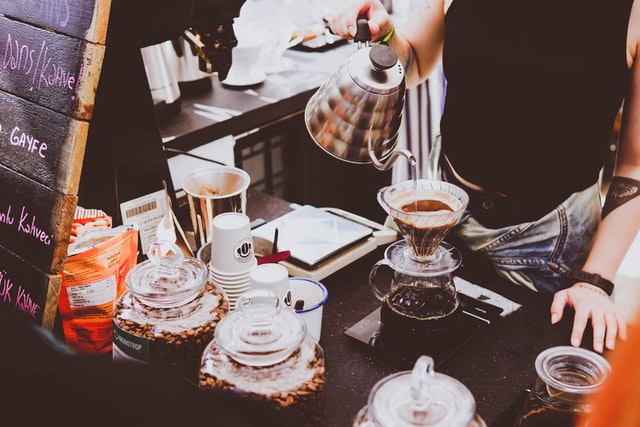
\includegraphics[scale=0.5]{sample}
\end{figure}

\begin{tikzpicture}
\begin{axis}[
    axis lines=left,
    xlabel=$x$,
    ylabel={$f(x)$},
]

\addplot [color=red]{x^2};
\addlegendentry{$x^2-2x-1$}
\end{axis}
\end{tikzpicture}


\bibliography{refs_contrastive}
\bibliographystyle{plain}

\end{document}